\documentclass{../../../oss-handout}
\usepackage{amsmath,bm}
\usepackage{txfonts}  % must be loaded after amsmath?
\usepackage{enumitem}
\usepackage{tikz}
\usepackage{siunitx}

\sisetup{
  detect-all,
  per-mode=symbol
}
\tikzset{>=latex}

%\usetikzlibrary{decorations.pathmorphing,patterns}

\setlength{\parindent}{0pt}
\setlength{\parskip}{8pt}
\setlength{\headheight}{26pt}

\newcommand{\mb}[1]{\ensuremath\mathbf{#1}}
\newcommand{\pic}[2]{\includegraphics[width=#1\textwidth]{#2}}

%\newcommand\vertarrowbox[2]{%
%    \begin{array}[t]{@{}c@{}} #1 \\
%    \rotatebox{90}{$\xrightarrow{\hphantom{abcdefgh}}$} \\[-1ex]
%    \mathclap{\scriptstyle\text{#2}}%
%    \end{array}}


% Set the page style for the document
\pagestyle{plain}

% Course & handout information
\renewcommand{\institution}{Olympiads School, Toronto, ON, Canada}
\renewcommand{\coursetitle}{Advanced Placement Physics C}
\renewcommand{\term}{Summer 2020}

\title{Kepler's Laws of Planetary Motion}
\author{Dr.\ Timothy Leung}
\date{\today}

\begin{document}
\thispagestyle{title}
\gentitle

Johannes Kepler\footnote{1571--1630. German mathematician, astromer and
  astrologer.} formulated his \textbf{laws of planetary motion}
between 1609 to 1619, by carefully interpreting the empirical planetary motion
data from his teacher, Tycho Brahe.\footnote{1546--1601. Danish nobleman and
  astronomer.} It is an improvement over the heliocentric
theory of Nicolaus Copernicus\footnote{1473--1543}. It should be noted that the
complete mathematical understanding was missing until Issac
Newton\footnote{1642--1726. English mathematician, physicist, astronomer,
  theologian, and author.} derived each law as pieces using his laws of motion.
In this handout we seek to obtain each law in turn, as we consider the orbit of
a small planet in the gravitational field of a much more massive star. In
modern form, Kepler's laws of planetary motion state that:
\begin{enumerate}[leftmargin=18pt,noitemsep,topsep=0pt]
\item A planet moves around the Sun in an elliptical path with the Sun as one
  of the foci.
\item The line segment joining a planet and the Sun sweeps out equal areas
  during equal intervals of time.
\item The square of the orbital time period of a planet is proportional to the
  cube of the semi-major axis of its orbit.
\end{enumerate}
To begin, we recognize that two properties of gravitational force, or Newton's
\textbf{law of universal gravitation}:
\begin{equation}
  \mb{F}_g=-\frac{Gm_1m_2}{r^2}\hat{\mb{r}}
\end{equation}
are crucial to
understanding orbital mechanics. These two properties hold true regardless
of the shape of the orbit, and whether an object is even in orbit altogether:
\begin{enumerate}[leftmargin=18pt,topsep=0pt]
\item Gravity is a \emph{conservative} force, in that
  \begin{itemize}[leftmargin=15pt,noitemsep,topsep=0pt]
  \item assuming that minor collisions with space dust and other methods of
    energy dissipation are negligible, then the total mechanical energy
    $E=K+U_g$ is conserved.
  \item work done \emph{by} gravity (positive work) converts gravitational
    potential energy $U_g$ into kinetic energy $K$, while work \emph{against}
    gravity (negative work) converts $K$ into $U_g$.
  \end{itemize}
\item Gravity is a \emph{central} force, in that
  \begin{itemize}[leftmargin=15pt,noitemsep,topsep=0pt]
  \item gravitational force $\mb{F}_g$ is always in the $-\hat{\mb{r}}$
    direction (i.e.\ $\mb{F}\times\mb{r}=\mb{0}$), shown in
    Fig.~\ref{central-force}, therefore gravity does not generate any torque,
  \item angular momentum $\mb{L}$ about the sun is therefore constant
  \end{itemize}
\end{enumerate}
\begin{figure}[!ht]
  \centering
  \begin{tikzpicture}[scale=1.3]
    \draw[->,ultra thick,blue](0,0)--(2,3)
    node[midway,left]{$\mb{r}$};
    \draw[->,thick](0,0)--(2,3) node[midway,left]{$\mb{r}$};
    \begin{scope}[rotate around={-33.7:(2.03,3)}]
      \draw[->,ultra thick,red](2.03,3)--(2.03,1.5)
      node[midway,below right]{$\mb{F}_g$};
    \end{scope}
    \draw[->,thick](2,3)--(3,2.8) node[pos=1,right]{$\mb{v}$};
    \fill[black](0,0) circle(.12) node[right]{\;Sun};
    \fill[black](2,3) circle(.07) node[left]{Planet\;};
  \end{tikzpicture}
  \caption{A central force such as gravity do not generate a torque (moment).}
  \label{central-force}
\end{figure}
For the purpose of the analysis, we assume that the Sun's mass $M_\odot$
is very large compared to any other object in the solar system (planets,
comets, asteroids, etc.), and its motion is essentially unaffected by the
gravity from them.

\section{Second law: Equal area in equal time}

The second law of planetary motion, called the \textbf{law of equal areas},
states (in modern terms) that line segment joining a planet and the Sun sweeps
out equal areas during equal intervals of time (Fig.~\ref{kep2}). The second
law of planetary motion is the easiest to proof using concepts in rotational
motion.
\begin{figure}[!ht]
  \centering
    \pic{.4}{../201532-132212364-3243-planet.png}
    \caption{The Earth sweeps out the same shaded area (purple) over the
      same amount of time regardless of where it is in its orbit.}
    \label{kep2}
\end{figure}

To begin, recognize that for a planet with a velocity vector $\mb{v}$ that is
not co-linear with the displacement vector $\mb{r}$ will sweep out an
infinitesimal area $d\mb{A}$ (Fig.~\ref{fig:dA})
\begin{figure}[ht]
  \centering
  \begin{tikzpicture}[scale=1.3]
    \fill[gray!45](0,0)--(2,3)--(3,2.8)--cycle;
    \node at (1.7,2) {$d\mb{A}$};
    \draw[->,thick](0,0)--(2,3)
    node[midway,left]{$\mb{r}$} node[pos=.95,right]{$\alpha$};
    \draw[->,thick](2,3)--(3,2.8) node[midway,above]{$d\mb{r}$};
    \draw[dashed](3,2.8)--(0,0);
    \fill[black](0,0) circle(.07) node[right]{Sun};
    \fill[black](2,3) circle(.035)node[left]{Planet};
  \end{tikzpicture}
  \caption{Infinitesimal area $d\mb{A}$ swept by a planet as it moves
    $d\mb{r}$ in orbit.}
  \label{fig:dA}
\end{figure}
as it moves in orbit by an infinitesimal amount $d\mb{r}$, which can be
computed by the area of the triangle:
\begin{equation}
  dA=\frac12rdr\sin\alpha
\end{equation}
or in vector form:
\begin{equation}
  d\mb{A}=\frac12\mb{r}\times d\mb{r}
\end{equation}
The direction of $d\mb{A}$, in this case, points into the
page.\footnote{The direction of the vector is not important in the calculation,
  but is only used to formalize the vector operations.} The time derivative of
the area is called the \textbf{areal velocity}, which literally means how
quickly the area is changing:
\begin{equation}
  \frac{d\mb{A}}{dt}
  =\frac12\mb{r}\times\frac{d\mb{r}}{dt}
  =\frac12\mb{r}\times\mb{v}
\end{equation}
We can express $\mb{r}\times\mb{v}$ in terms of angular momentum. Since angular
momentum is defined as $\mb{L}=m(\mb{r}\times\mb{v})\;\rightarrow\;
\mb{r}\times\mb{v}=\mb{L}/m$. Since gravity is a central force, angular
momentum is a constant, i.e:
\begin{equation}
  \boxed{\frac{d\mb{A}}{dt}
    =\frac12(\mb{r}\times\mb{v})=\frac{\mb{L}}{2m}=
    \text{constant}
  }
  \label{constant}
\end{equation}
as predicted by Kepler's second law. The rate that a planet sweeps out the area
in orbit is its angular momentum around the sun, divided by twice its mass. It
is constant regardless of its location relative to the sun.

\section{First Law: The Law of Ellipses}
Kepler's first law, called the \textbf{law of ellipses}, is more difficult to
proof. In order to proof the
law, we must show that all orbital motion must agree with the equations of an
ellipse. An ellipse is shown in Fig.~\ref{ellipse1} with the origin of the
coordinate system located at one of the two foci.
\begin{figure}[!ht]
  \centering
  \begin{tikzpicture}
    \def\a{4}       % semi-major axis
    \def\b{3.25}    % semi-minor axis
    \def\angle{150} % angle
    \draw[thick] (0,0) ellipse ({\a} and {\b});% Draw the ellipse
    \draw[->] ({sqrt(\a*\a-\b*\b)},-3.5)--({sqrt(\a*\a-\b*\b)},3.5)
    node[pos=1,above]{$y$};
    \draw[->] (-\a-.2,0)--(\a+.5,0) node[pos=1,right]{$x$};
    \begin{scope}[rotate around={\angle:({sqrt(\a*\a-\b*\b)},0)}]
      \draw[red,thick]({sqrt(\a*\a-\b*\b)},0)--(7.66,0) node[pos=.7,below]{$r$};
      \fill[red] (7.66,0) circle(.04);
    \end{scope}
    \begin{scope}[rotate around={-91.1:({-sqrt(\a*\a-\b*\b)},0)}]
      \draw[red,thick]({-sqrt(\a*\a-\b*\b)},0)--(-5,0) node[midway,left]{$r'$};
    \end{scope}
    \draw[->]({sqrt(\a*\a-\b*\b)+.5},0) arc(0:\angle:.5)
    node[pos=.4,above]{$\theta$};
    %\draw[<->]({sqrt(\a*\a-\b*\b)-.2},0)--({sqrt(\a*\a-\b*\b)-.2},-2.65)
    %node[midway,left]{\tiny$r_0$};
    \fill ({sqrt(\a*\a-\b*\b)},0) circle(.05) node[below]{$f_1$};
    \fill ({-sqrt(\a*\a-\b*\b)},0) circle(.05) node[below]{$f_2$};
    \draw[very thick, blue](0,0)--(\a,0) node[midway,below]{$a$};
    \draw[very thick, blue](0,0)--(-\a,0) node[midway,below]{$a$};
    \draw[very thick, green](0,0)--(0,\b) node[midway,right]{$b$};
    \draw[very thick, green](0,0)--(0,-\b) node[midway,right]{$b$};
  \end{tikzpicture}
  \caption{A basic ellipse with the origin of the coordinate system placed at
    one of the focus.}
  \label{ellipse1}
\end{figure}

The longest dimension from the origin is the \textbf{semi-major axis} $a$, while
the shortest dimension is the \textbf{semi-minor axis} $b$. The two lengths are
related by the parameter $e$, generally called the \textbf{eccentricity} of the
ellipse:
\begin{equation}
  b^2=a^2(1-e^2)\quad\text{where}\quad 0\leq e < 1
\end{equation}
When the eccentricity of a planet's orbit is zero, the orbit is perfectly
circular, and $a=b=r$. As $e\rightarrow 1$, the orbit is stretched out into
more elongated elliptical trajectories.
%To illustrate this, orbits with different values of $e$ are plotted in
%Fig.~\ref{eccentricity}.
At $e=1$, the shape becomes a parabola, and is no longer an ellipse.
%\begin{figure}[!ht]
%  \centering
%  \caption{Plot of the orbits for increasing eccentricity}
%  \label{eccentricity}
%\end{figure}

The area $A$ of an ellipse is given by the semi-major and semi-minor axes:
\begin{equation}
  A=\pi ab=\pi a^2\sqrt{1-e^2}
  \label{A2}
\end{equation}
When the origin of the coordinate system placed one of the two foci, an ellipse
can be expressed using polar coordinates:
\begin{equation}
  r=\frac{a(1-e^2)}{1+e\cos\theta}
  \label{ellipse-eq}
\end{equation}

As shown in Fig.~\ref{eorbit}, there are two components of velocity when a
planet orbits a star:
\begin{figure}[!ht]
  \centering
  \begin{tikzpicture}[scale=.8]
    \def\a{4}       % semi-major axis
    \def\b{3.25}    % semi-minor axis
    \def\angle{150} % angle
    \draw[very thick] (0,0) ellipse ({\a} and {\b});% Draw the ellipse
    \draw ({sqrt(\a*\a-\b*\b)},-2.65)--({sqrt(\a*\a-\b*\b)},2.65);
    \draw (-\a-.2,0)--(\a+.2,0);
    \fill[black]({sqrt(\a*\a-\b*\b)},0) circle(.1) node[below right]{$M$};
    \begin{scope}[rotate around={\angle:({sqrt(\a*\a-\b*\b)},0)}]
      \draw[->]({sqrt(\a*\a-\b*\b)},0)--(8.5,0)
      node[pos=.45,below]{$\mb{r}$} node[pos=1,left]{$\mb{v}_r$};
      \draw[->](7.65,0)--(7.65,.85) node[below]{$\mb{v}_\theta$};
      \fill (7.65,0) circle(.1) node[above]{$m$};
    \end{scope}
    \draw[->]({sqrt(\a*\a-\b*\b)+.5},0) arc(0:\angle:.5)
    node[pos=.4,above]{$\theta$};
  \end{tikzpicture}
  \caption{Elliptical orbit of a small mass $m$ around a large mass $M$.}
  \label{eorbit}
\end{figure}
\begin{itemize}[leftmargin=15pt]
\item\textbf{Angular velocity} $\mb{v}_\theta$. The presence of $\mb{v}_\theta$
  means that there is a centripetal acceleration $a_c$ toward $M$. The
  direction of the acceleration is perpendicular to the direction of
  $\mb{v}_\theta$, and towards the sun:
  \begin{equation}
    a_c=-r\omega^2\hat{\mb{r}}
  \end{equation}
\item\textbf{Radial velocity} $\mb{v}_r$. If this velocity is non-zero and
  changes with time (which is the case for elliptical orbits but not for
  circular orbits), then there is an acceleration $a_r$, also in the radial
  direction:
  \begin{equation}
    a_r=\frac{dv_r}{dt}\hat{\mb{r}}=\frac{d^2r}{dt^2}\hat{\mb{r}}
  \end{equation}
\end{itemize}
Both components of acceleration are due entirely to gravitational force.
Applying second law of motion ($\sum F=ma$), and dividing all sides by the mass
of the planet $m$, we arrive at a differential equation:
\begin{equation}
  \frac{d^2r}{dt^2}-r\omega^2=-\frac{GM}{r^2}
  \label{ode1}
\end{equation}
In this equation, the ($+$) direction is radially outward from $M$. In the
circular motion case, where $\ddot{r}=0$, we are left with only the centripetal
acceleration
$a_c=r\omega^2$ which is expected in uniform circular motion. The differential
equation, in its present form, is difficult to solve. Moreover, the equation
that for an ellipse (Eq.~\ref{ellipse-eq}) depends on $\theta$ but not on $t$.
However, the
differential equation is easier to solve by making a variable
substitution\footnote{this variable may not be immediately obvious without
  some experience with solving ODEs}, by introducing a new variable $u$ which
is the inverse of the radius $r$:
\begin{equation}
  u=\frac1r
\end{equation}
We can then use the fact that angular momentum $L$ is constant to relate
derivatives in time $t$ to derivatives in angle $\theta$:
\begin{equation}
  L=mr^2\frac{d\theta}{dt}=\frac{m}{u^2}\frac{d\theta}{dt}
  \quad\longrightarrow\quad
  \frac{d}{d\theta}=\frac{Lu^2}{m}\frac{d}{dt}
\end{equation}
The derivative $\dot{r}$ can now be expressed in terms of derivatives of
$\theta$ instead of time $t$:
\begin{align}
  \nonumber
  \frac{dr}{dt} &=\frac{d}{dt}\left(\frac{1}{u}\right)
  =-\frac{1}{u}\frac{du}{dt}\\
  \nonumber
  &=-\frac{L}{m}\frac{du}{d\theta}\\
  \nonumber
  &= -u^{-2}\frac{du}{d\theta} \frac{Lu^2}{m} \\
  \frac{dr}{dt}&= -\frac{L}{m}\frac{du}{d\theta}
\end{align}
Repeating the same process for the second derivative $\ddot{r}$, we have
\begin{align}
  \nonumber
  \frac{d^2r}{dt^2} &= \frac{d}{dt}\left(-\frac{L}{m}\frac{du}{d\theta}\right)\\
  \nonumber
  &= -\frac{L}{m} \frac{d}{d\theta}\frac{du}{d\theta} \\
  \frac{d^2r}{dt^2}&= -\left(\frac{L^2u^2}{m^2}\right)\frac{d^2u}{d\theta^2}
\end{align}
With this identity in hand, our original differential equation
(Eq.~\ref{ode1}) becomes
\begin{equation}
  -\left(\frac{L^2u^2}{m^2}\right)\frac{d^2u}{d\theta^2} - \left(\frac{L}{m}\right)^2u^3 = -GMu^2
\end{equation}
which can be simplified to:
\begin{equation}
  \frac{d^2u}{d\theta^2} + u = \frac{GMm^2}{L^2}
  \label{newdiff}
\end{equation}
Anyone experienced with calculus can recognize that Eq.\ \ref{newdiff} is a
\emph{second-order ordinary differential equation with constant coefficients
  and a constant forcing function}. The solution to this type of equation is in
the form
\begin{equation} 
  u =B\cos\theta + \frac{GMm^2}{L^2}
\end{equation}
where the coefficient $B$ is determined by the total energy and total angular
momentum (both are constants) of the planets. Solving for $r=1/u$, we have
\begin{equation}
  r(\theta)=\frac1u = \frac1{B\cos\theta+ \frac{GMm^2}{L^2}}
  =\left(\frac{L^2}{GMm^2}\right)\frac1{1+e\cos\theta}
\end{equation}
where $e$ is a constant:
\begin{equation}
  e=\dfrac{BL^2}{GMm^2}
\end{equation}
It should become obvious that this $e$ is, in fact, the eccentricity of the
elliptical orbit previously mentioned. If a planet, or any celestrial object
has too much total energy when it enters the gravitational field of the sun,
then $e>1$, and the object will not return.
From this form of $r$, it is clear that the maximum and a
minimum values of $r$ represent the \emph{aphelion} and \emph{perihelion} of
an ellipse (points of furthest and closest distance to the focus):
\begin{equation}
  r_\text{max}=\left(\frac{L^2}{GMm^2}\right)\frac1{1-e}
  \quad\quad
  r_\text{min}=\left(\frac{L^2}{GMm^2}\right)\frac1{1+e}
\end{equation}
This the semi-major axis $r$ is the average of the two values:
\begin{equation}
  a=\dfrac12\left(r_\text{min} + r_\text{max}\right)=
  \left(\frac{L^2}{GMm^2}\right)\frac1{1-e^2}
  \label{semimajor}
\end{equation}
More importantly, Eq.\ \ref{semimajor} allows us to relate the eccentricity
$e$ and the semi-major axis $a$ to the numerator in the $r$ expression:
\begin{equation}
  a(1-e^2)=\frac{L^2}{GMm^2}
  \label{eq:numerator}
\end{equation}
We see that the orbit is given by an ellipse as Kepler found from Brahe's
data. Moreover, since $r_\mathrm{min}$ and $r_\mathrm{max}$ are distances from
the Sun, we see that the Sun is at one focus of the orbit. Thus, we have
derived Kepler's first law.

\section{Third law: Period of motion}
\begin{figure}[!ht]
  \centering
  \pic{.55}{../kep8.png}
  \caption{The orbits of all the planets in the solar system obey the third
  law of planetary motion.}
  \label{3rdlaw}
\end{figure}
In the third law, called the \textbf{law of periods}, the total area $A$
swept by the planet through one orbital period is the areal velocity (which is
constant, as shown in Eq.\ \ref{constant}) integrated by time, from $t=0$ to
$T$, the orbital period of the planet:
\begin{equation}
  A=\int dA=\int_0^T\frac{dA}{dt}dt=\frac{L}{2m}\int_0^Tdt=\frac{LT}{2m}
  \label{A1}
\end{equation}
From proofing Kepler's first law in the previous section, we know that the
area $A$ is in the form of an ellipse, given in Eq.~\ref{A2}. Solving for
period $T$ in Eq.~\ref{A1}, then substituting the expression for area from
Eq.~\ref{A2}, and then squaring both sides, we arrive at this expression:
\begin{equation}
  T^2=\frac{m^2}{L^2}4\pi^2a^4(1-e^2)
  \label{eq:almost}
\end{equation}
Substituting Eq.~\ref{eq:numerator}
%, shown below for reference:
%\begin{displaymath}
%  a(1-e^2)=\frac{L^2}{GMm^2}
%\end{displaymath}
into Eq.\ \ref{eq:almost} above, and after some simple algebra, we arrive at
this expression:
\begin{equation}
  \boxed{T^2=\left[\frac{4\pi^2}{GM}\right] a^3}
\end{equation}
which is Kepler's third law. Note that this law holds for all elliptical
orbits, regardless of their eccentricities.
\end{document}
